% Options for packages loaded elsewhere
\PassOptionsToPackage{unicode}{hyperref}
\PassOptionsToPackage{hyphens}{url}
\PassOptionsToPackage{dvipsnames,svgnames,x11names}{xcolor}
%
\documentclass[
  letterpaper,
  DIV=11,
  numbers=noendperiod]{scrartcl}

\usepackage{amsmath,amssymb}
\usepackage{iftex}
\ifPDFTeX
  \usepackage[T1]{fontenc}
  \usepackage[utf8]{inputenc}
  \usepackage{textcomp} % provide euro and other symbols
\else % if luatex or xetex
  \usepackage{unicode-math}
  \defaultfontfeatures{Scale=MatchLowercase}
  \defaultfontfeatures[\rmfamily]{Ligatures=TeX,Scale=1}
\fi
\usepackage{lmodern}
\ifPDFTeX\else  
    % xetex/luatex font selection
\fi
% Use upquote if available, for straight quotes in verbatim environments
\IfFileExists{upquote.sty}{\usepackage{upquote}}{}
\IfFileExists{microtype.sty}{% use microtype if available
  \usepackage[]{microtype}
  \UseMicrotypeSet[protrusion]{basicmath} % disable protrusion for tt fonts
}{}
\makeatletter
\@ifundefined{KOMAClassName}{% if non-KOMA class
  \IfFileExists{parskip.sty}{%
    \usepackage{parskip}
  }{% else
    \setlength{\parindent}{0pt}
    \setlength{\parskip}{6pt plus 2pt minus 1pt}}
}{% if KOMA class
  \KOMAoptions{parskip=half}}
\makeatother
\usepackage{xcolor}
\setlength{\emergencystretch}{3em} % prevent overfull lines
\setcounter{secnumdepth}{-\maxdimen} % remove section numbering
% Make \paragraph and \subparagraph free-standing
\makeatletter
\ifx\paragraph\undefined\else
  \let\oldparagraph\paragraph
  \renewcommand{\paragraph}{
    \@ifstar
      \xxxParagraphStar
      \xxxParagraphNoStar
  }
  \newcommand{\xxxParagraphStar}[1]{\oldparagraph*{#1}\mbox{}}
  \newcommand{\xxxParagraphNoStar}[1]{\oldparagraph{#1}\mbox{}}
\fi
\ifx\subparagraph\undefined\else
  \let\oldsubparagraph\subparagraph
  \renewcommand{\subparagraph}{
    \@ifstar
      \xxxSubParagraphStar
      \xxxSubParagraphNoStar
  }
  \newcommand{\xxxSubParagraphStar}[1]{\oldsubparagraph*{#1}\mbox{}}
  \newcommand{\xxxSubParagraphNoStar}[1]{\oldsubparagraph{#1}\mbox{}}
\fi
\makeatother

\usepackage{color}
\usepackage{fancyvrb}
\newcommand{\VerbBar}{|}
\newcommand{\VERB}{\Verb[commandchars=\\\{\}]}
\DefineVerbatimEnvironment{Highlighting}{Verbatim}{commandchars=\\\{\}}
% Add ',fontsize=\small' for more characters per line
\usepackage{framed}
\definecolor{shadecolor}{RGB}{241,243,245}
\newenvironment{Shaded}{\begin{snugshade}}{\end{snugshade}}
\newcommand{\AlertTok}[1]{\textcolor[rgb]{0.68,0.00,0.00}{#1}}
\newcommand{\AnnotationTok}[1]{\textcolor[rgb]{0.37,0.37,0.37}{#1}}
\newcommand{\AttributeTok}[1]{\textcolor[rgb]{0.40,0.45,0.13}{#1}}
\newcommand{\BaseNTok}[1]{\textcolor[rgb]{0.68,0.00,0.00}{#1}}
\newcommand{\BuiltInTok}[1]{\textcolor[rgb]{0.00,0.23,0.31}{#1}}
\newcommand{\CharTok}[1]{\textcolor[rgb]{0.13,0.47,0.30}{#1}}
\newcommand{\CommentTok}[1]{\textcolor[rgb]{0.37,0.37,0.37}{#1}}
\newcommand{\CommentVarTok}[1]{\textcolor[rgb]{0.37,0.37,0.37}{\textit{#1}}}
\newcommand{\ConstantTok}[1]{\textcolor[rgb]{0.56,0.35,0.01}{#1}}
\newcommand{\ControlFlowTok}[1]{\textcolor[rgb]{0.00,0.23,0.31}{\textbf{#1}}}
\newcommand{\DataTypeTok}[1]{\textcolor[rgb]{0.68,0.00,0.00}{#1}}
\newcommand{\DecValTok}[1]{\textcolor[rgb]{0.68,0.00,0.00}{#1}}
\newcommand{\DocumentationTok}[1]{\textcolor[rgb]{0.37,0.37,0.37}{\textit{#1}}}
\newcommand{\ErrorTok}[1]{\textcolor[rgb]{0.68,0.00,0.00}{#1}}
\newcommand{\ExtensionTok}[1]{\textcolor[rgb]{0.00,0.23,0.31}{#1}}
\newcommand{\FloatTok}[1]{\textcolor[rgb]{0.68,0.00,0.00}{#1}}
\newcommand{\FunctionTok}[1]{\textcolor[rgb]{0.28,0.35,0.67}{#1}}
\newcommand{\ImportTok}[1]{\textcolor[rgb]{0.00,0.46,0.62}{#1}}
\newcommand{\InformationTok}[1]{\textcolor[rgb]{0.37,0.37,0.37}{#1}}
\newcommand{\KeywordTok}[1]{\textcolor[rgb]{0.00,0.23,0.31}{\textbf{#1}}}
\newcommand{\NormalTok}[1]{\textcolor[rgb]{0.00,0.23,0.31}{#1}}
\newcommand{\OperatorTok}[1]{\textcolor[rgb]{0.37,0.37,0.37}{#1}}
\newcommand{\OtherTok}[1]{\textcolor[rgb]{0.00,0.23,0.31}{#1}}
\newcommand{\PreprocessorTok}[1]{\textcolor[rgb]{0.68,0.00,0.00}{#1}}
\newcommand{\RegionMarkerTok}[1]{\textcolor[rgb]{0.00,0.23,0.31}{#1}}
\newcommand{\SpecialCharTok}[1]{\textcolor[rgb]{0.37,0.37,0.37}{#1}}
\newcommand{\SpecialStringTok}[1]{\textcolor[rgb]{0.13,0.47,0.30}{#1}}
\newcommand{\StringTok}[1]{\textcolor[rgb]{0.13,0.47,0.30}{#1}}
\newcommand{\VariableTok}[1]{\textcolor[rgb]{0.07,0.07,0.07}{#1}}
\newcommand{\VerbatimStringTok}[1]{\textcolor[rgb]{0.13,0.47,0.30}{#1}}
\newcommand{\WarningTok}[1]{\textcolor[rgb]{0.37,0.37,0.37}{\textit{#1}}}

\providecommand{\tightlist}{%
  \setlength{\itemsep}{0pt}\setlength{\parskip}{0pt}}\usepackage{longtable,booktabs,array}
\usepackage{calc} % for calculating minipage widths
% Correct order of tables after \paragraph or \subparagraph
\usepackage{etoolbox}
\makeatletter
\patchcmd\longtable{\par}{\if@noskipsec\mbox{}\fi\par}{}{}
\makeatother
% Allow footnotes in longtable head/foot
\IfFileExists{footnotehyper.sty}{\usepackage{footnotehyper}}{\usepackage{footnote}}
\makesavenoteenv{longtable}
\usepackage{graphicx}
\makeatletter
\def\maxwidth{\ifdim\Gin@nat@width>\linewidth\linewidth\else\Gin@nat@width\fi}
\def\maxheight{\ifdim\Gin@nat@height>\textheight\textheight\else\Gin@nat@height\fi}
\makeatother
% Scale images if necessary, so that they will not overflow the page
% margins by default, and it is still possible to overwrite the defaults
% using explicit options in \includegraphics[width, height, ...]{}
\setkeys{Gin}{width=\maxwidth,height=\maxheight,keepaspectratio}
% Set default figure placement to htbp
\makeatletter
\def\fps@figure{htbp}
\makeatother

\usepackage{fvextra}
\DefineVerbatimEnvironment{Highlighting}{Verbatim}{breaklines,commandchars=\\\{\}}
\KOMAoption{captions}{tableheading}
\makeatletter
\@ifpackageloaded{caption}{}{\usepackage{caption}}
\AtBeginDocument{%
\ifdefined\contentsname
  \renewcommand*\contentsname{Table of contents}
\else
  \newcommand\contentsname{Table of contents}
\fi
\ifdefined\listfigurename
  \renewcommand*\listfigurename{List of Figures}
\else
  \newcommand\listfigurename{List of Figures}
\fi
\ifdefined\listtablename
  \renewcommand*\listtablename{List of Tables}
\else
  \newcommand\listtablename{List of Tables}
\fi
\ifdefined\figurename
  \renewcommand*\figurename{Figure}
\else
  \newcommand\figurename{Figure}
\fi
\ifdefined\tablename
  \renewcommand*\tablename{Table}
\else
  \newcommand\tablename{Table}
\fi
}
\@ifpackageloaded{float}{}{\usepackage{float}}
\floatstyle{ruled}
\@ifundefined{c@chapter}{\newfloat{codelisting}{h}{lop}}{\newfloat{codelisting}{h}{lop}[chapter]}
\floatname{codelisting}{Listing}
\newcommand*\listoflistings{\listof{codelisting}{List of Listings}}
\makeatother
\makeatletter
\makeatother
\makeatletter
\@ifpackageloaded{caption}{}{\usepackage{caption}}
\@ifpackageloaded{subcaption}{}{\usepackage{subcaption}}
\makeatother

\ifLuaTeX
  \usepackage{selnolig}  % disable illegal ligatures
\fi
\usepackage{bookmark}

\IfFileExists{xurl.sty}{\usepackage{xurl}}{} % add URL line breaks if available
\urlstyle{same} % disable monospaced font for URLs
\hypersetup{
  pdftitle={Amulya Jasti PS4},
  colorlinks=true,
  linkcolor={blue},
  filecolor={Maroon},
  citecolor={Blue},
  urlcolor={Blue},
  pdfcreator={LaTeX via pandoc}}


\title{Amulya Jasti PS4}
\author{}
\date{}

\begin{document}
\maketitle

\RecustomVerbatimEnvironment{verbatim}{Verbatim}{
  showspaces = false,
  showtabs = false,
  breaksymbolleft={},
  breaklines
}


\textbf{PS4:} Due Sat Nov 2 at 5:00PM Central. Worth 100 points. We use
(\texttt{*}) to indicate a problem that we think might be time
consuming.

\subsection{Style Points (10 pts)}\label{style-points-10-pts}

Please refer to the minilesson on code style
\textbf{\href{https://uchicago.zoom.us/rec/share/pG_wQ-pHTQrJTmqNn4rcrw5V194M2H2s-2jdy8oVhWHkd_yZt9o162IWurpA-fxU.BIQlSgZLRYctvzp-}{here}}.

\subsection{Submission Steps (10 pts)}\label{submission-steps-10-pts}

\begin{enumerate}
\def\labelenumi{\arabic{enumi}.}
\tightlist
\item
  This problem set is a paired problem set.
\item
  Play paper, scissors, rock to determine who goes first. Call that
  person \emph{Partner 1}.

  \begin{itemize}
  \tightlist
  \item
    Partner 1 (name and cnet ID): Amulya Jasti amulyaj
  \item
    Partner 2 (name and cnet ID): Amulya Jasti amulyaj
  \end{itemize}
\item
  Partner 1 will accept the \texttt{ps4} and then share the link it
  creates with their partner. You can only share it with one partner so
  you will not be able to change it after your partner has accepted.
\item
  ``This submission is our work alone and complies with the 30538
  integrity policy.'' Add your initials to indicate your agreement: AJ
\item
  ``I have uploaded the names of anyone else other than my partner and I
  worked with on the problem set
  \textbf{\href{https://docs.google.com/forms/d/185usrCREQaUbvAXpWhChkjghdGgmAZXA3lPWpXLLsts/edit}{here}}''
  (1 point) AJ
\item
  Late coins used this pset: 1 Late coins left after submission: 3
\item
  Knit your \texttt{ps4.qmd} to an PDF file to make \texttt{ps4.pdf},

  \begin{itemize}
  \tightlist
  \item
    The PDF should not be more than 25 pages. Use \texttt{head()} and
    re-size figures when appropriate.
  \end{itemize}
\item
  (Partner 1): push \texttt{ps4.qmd} and \texttt{ps4.pdf} to your github
  repo.
\item
  (Partner 1): submit \texttt{ps4.pdf} via Gradescope. Add your partner
  on Gradescope.
\item
  (Partner 1): tag your submission in Gradescope
\end{enumerate}

\textbf{Important:} Repositories are for tracking code. \textbf{Do not
commit the data or shapefiles to your repo.} The best way to do this is
with \texttt{.gitignore}, which we have covered in class. If you do
accidentally commit the data, Github has a
\href{https://docs.github.com/en/repositories/working-with-files/managing-large-files/about-large-files-on-github\#removing-files-from-a-repositorys-history}{guide}.
The best course of action depends on whether you have pushed yet. This
also means that both partners will have to download the initial raw data
and any data cleaning code will need to be re-run on both partners'
computers.

\begin{Shaded}
\begin{Highlighting}[]
\ImportTok{import}\NormalTok{ pandas }\ImportTok{as}\NormalTok{ pd}
\ImportTok{import}\NormalTok{ altair }\ImportTok{as}\NormalTok{ alt}
\NormalTok{alt.renderers.enable(}\StringTok{"png"}\NormalTok{)}
\NormalTok{alt.data\_transformers.disable\_max\_rows()}
\ImportTok{import}\NormalTok{ time}
\ImportTok{import}\NormalTok{ numpy }\ImportTok{as}\NormalTok{ np}

\ImportTok{import}\NormalTok{ warnings }
\NormalTok{warnings.filterwarnings(}\StringTok{\textquotesingle{}ignore\textquotesingle{}}\NormalTok{)}
\end{Highlighting}
\end{Shaded}

\subsection{Download and explore the Provider of Services (POS) file (10
pts)}\label{download-and-explore-the-provider-of-services-pos-file-10-pts}

\begin{enumerate}
\def\labelenumi{\arabic{enumi}.}
\item
  I downloaded the following variables: PRVDR\_CTGRY\_SBTYP\_CD
  (provider subtype code), PRVDR\_CTGRY\_CD (provider type code),
  FAC\_NAME (facility name), PRVDR\_NUM (CMS certification number),
  PGM\_TRMNTN\_CD (termination code), and ZIP\_CD (zip code).
\item
  \begin{enumerate}
  \def\labelenumii{\alph{enumii}.}
  \tightlist
  \item
    There are 7245 observations in the subsetted data. This makes sense,
    although it intially seems a little large, because these span the
    United States and are only short-term providers (requiring fewer
    resources and serving fewer people).
  \end{enumerate}
\end{enumerate}

\begin{Shaded}
\begin{Highlighting}[]
\NormalTok{my\_path }\OperatorTok{=} \VerbatimStringTok{r\textquotesingle{}C:\textbackslash{}Users\textbackslash{}amuly\textbackslash{}OneDrive\textbackslash{}Documents\textbackslash{}GitHub\textbackslash{}Python2{-}PS4\textquotesingle{}}
\NormalTok{pos2016 }\OperatorTok{=}\NormalTok{ pd.read\_csv(my\_path }\OperatorTok{+} \StringTok{\textquotesingle{}\textbackslash{}pos2016.csv\textquotesingle{}}\NormalTok{)  }\CommentTok{\# Read in csv.}
\NormalTok{pos2016 }\OperatorTok{=}\NormalTok{ pos2016.loc[(pos2016[}\StringTok{\textquotesingle{}PRVDR\_CTGRY\_SBTYP\_CD\textquotesingle{}}\NormalTok{] }\OperatorTok{==} \DecValTok{1}\NormalTok{) }\OperatorTok{\&}\NormalTok{ (}
\NormalTok{    pos2016[}\StringTok{\textquotesingle{}PRVDR\_CTGRY\_CD\textquotesingle{}}\NormalTok{] }\OperatorTok{==} \DecValTok{1}\NormalTok{)]  }\CommentTok{\# subset type and subtype codes of 1}
\BuiltInTok{print}\NormalTok{(}\BuiltInTok{len}\NormalTok{(pos2016))  }\CommentTok{\# number of observations}
\end{Highlighting}
\end{Shaded}

\begin{verbatim}
7245
\end{verbatim}

\begin{verbatim}
b. The Kaiser Family Foundation article from 2016 says "There are nearly 5,000 short-term, acute care hospitals in the United States." It also discusses how many are closing down at increasing rates. It could be that around 2000 of the short-term providers are not for acute care, or that there are differing definitions of the United States (ex. with or without territories). It could still make sense that in 2016 there were 7245 short-term providers in the dataset, but many have closed or were temporarily closed. 
\end{verbatim}

\begin{enumerate}
\def\labelenumi{\arabic{enumi}.}
\setcounter{enumi}{2}
\tightlist
\item
\end{enumerate}

\begin{Shaded}
\begin{Highlighting}[]
\NormalTok{pos2016[}\StringTok{\textquotesingle{}YEAR\textquotesingle{}}\NormalTok{] }\OperatorTok{=} \DecValTok{2016}  \CommentTok{\# added new col YEAR}
\NormalTok{pos\_combined }\OperatorTok{=}\NormalTok{ pos2016  }\CommentTok{\# new df with all years}
\ControlFlowTok{for}\NormalTok{ year }\KeywordTok{in}\NormalTok{ [}\StringTok{\textquotesingle{}2017\textquotesingle{}}\NormalTok{, }\StringTok{\textquotesingle{}2018\textquotesingle{}}\NormalTok{, }\StringTok{\textquotesingle{}2019\textquotesingle{}}\NormalTok{]:  }\CommentTok{\# looping to import other data}
    \CommentTok{\# import; error resolved with encoding from ChatGPT}
\NormalTok{    data }\OperatorTok{=}\NormalTok{ pd.read\_csv(my\_path }\OperatorTok{+} \SpecialStringTok{f\textquotesingle{}\textbackslash{}pos}\SpecialCharTok{\{}\NormalTok{year}\SpecialCharTok{\}}\SpecialStringTok{.csv\textquotesingle{}}\NormalTok{, encoding }\OperatorTok{=} \StringTok{\textquotesingle{}ISO{-}8859{-}1\textquotesingle{}}\NormalTok{)}
\NormalTok{    data }\OperatorTok{=}\NormalTok{ data.loc[(data[}\StringTok{\textquotesingle{}PRVDR\_CTGRY\_SBTYP\_CD\textquotesingle{}}\NormalTok{] }\OperatorTok{==} \DecValTok{1}\NormalTok{) }\OperatorTok{\&}\NormalTok{ (}
\NormalTok{        data[}\StringTok{\textquotesingle{}PRVDR\_CTGRY\_CD\textquotesingle{}}\NormalTok{] }\OperatorTok{==} \DecValTok{1}\NormalTok{)]  }\CommentTok{\# subset to type and subtype 1}
\NormalTok{    data[}\StringTok{\textquotesingle{}YEAR\textquotesingle{}}\NormalTok{] }\OperatorTok{=} \BuiltInTok{int}\NormalTok{(year)  }\CommentTok{\# add YEAR col}
    \CommentTok{\# append data to combined}
\NormalTok{    pos\_combined }\OperatorTok{=}\NormalTok{ pd.concat([pos\_combined, data], ignore\_index}\OperatorTok{=}\VariableTok{True}\NormalTok{)}


\NormalTok{chart\_count }\OperatorTok{=}\NormalTok{ alt.Chart(pos\_combined).mark\_bar().encode(}
\NormalTok{    alt.X(}\StringTok{\textquotesingle{}YEAR:N\textquotesingle{}}\NormalTok{, title }\OperatorTok{=} \StringTok{\textquotesingle{}Year\textquotesingle{}}\NormalTok{),}
\NormalTok{    alt.Y(}\StringTok{\textquotesingle{}count():Q\textquotesingle{}}\NormalTok{, title }\OperatorTok{=} \StringTok{\textquotesingle{}Number of observations\textquotesingle{}}\NormalTok{,}
\NormalTok{          scale}\OperatorTok{=}\NormalTok{alt.Scale(domain }\OperatorTok{=}\NormalTok{ [}\DecValTok{7000}\NormalTok{, }\DecValTok{7500}\NormalTok{]))}
\NormalTok{).properties(}
\NormalTok{        title}\OperatorTok{=}\SpecialStringTok{f\textquotesingle{}Number of observations across datasets\textquotesingle{}}
\NormalTok{    )}

\NormalTok{labels\_count }\OperatorTok{=}\NormalTok{ chart\_count.mark\_text(}
\NormalTok{    dx }\OperatorTok{=} \OperatorTok{{-}}\DecValTok{20}\NormalTok{,}
\NormalTok{    angle }\OperatorTok{=} \DecValTok{90}
\NormalTok{).encode(}
\NormalTok{    text }\OperatorTok{=}\NormalTok{ alt.Text(}\StringTok{\textquotesingle{}count():Q\textquotesingle{}}\NormalTok{)  }\CommentTok{\# Display the count on each bar}
\NormalTok{)  }\CommentTok{\# charting num of observations by YEAR}
\NormalTok{chart\_count }\OperatorTok{+}\NormalTok{ labels\_count}
\end{Highlighting}
\end{Shaded}

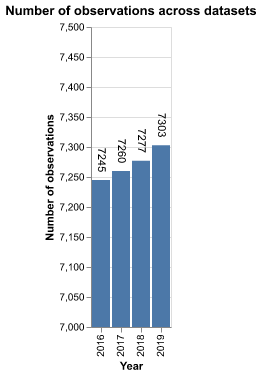
\includegraphics[width=2.72917in,height=3.92708in]{pset4_template_files/figure-pdf/cell-4-output-1.png}

\begin{enumerate}
\def\labelenumi{\arabic{enumi}.}
\setcounter{enumi}{3}
\tightlist
\item
  \begin{enumerate}
  \def\labelenumii{\alph{enumii}.}
  \tightlist
  \item
  \end{enumerate}
\end{enumerate}

\begin{Shaded}
\begin{Highlighting}[]
\NormalTok{chart\_unique }\OperatorTok{=}\NormalTok{ alt.Chart(pos\_combined).mark\_bar().encode(}
\NormalTok{    alt.X(}\StringTok{\textquotesingle{}YEAR:N\textquotesingle{}}\NormalTok{, title }\OperatorTok{=} \StringTok{\textquotesingle{}Year\textquotesingle{}}\NormalTok{),}
\NormalTok{    alt.Y(}\StringTok{\textquotesingle{}distinct(PRVDR\_NUM):Q\textquotesingle{}}\NormalTok{, title }\OperatorTok{=} \StringTok{\textquotesingle{}Number of unique observations\textquotesingle{}}\NormalTok{, scale}\OperatorTok{=}\NormalTok{alt.Scale(domain }\OperatorTok{=}\NormalTok{ [}\DecValTok{7000}\NormalTok{, }\DecValTok{7500}\NormalTok{]))}
\NormalTok{).properties(}
\NormalTok{        title}\OperatorTok{=}\SpecialStringTok{f\textquotesingle{}Number of unique observations across datasets\textquotesingle{}}
\NormalTok{    )}

\NormalTok{labels\_unique }\OperatorTok{=}\NormalTok{ chart\_unique.mark\_text(}
\NormalTok{    dx }\OperatorTok{=} \OperatorTok{{-}}\DecValTok{20}\NormalTok{,}
\NormalTok{    angle }\OperatorTok{=} \DecValTok{90}
\NormalTok{).encode(}
\NormalTok{    text }\OperatorTok{=}\NormalTok{ alt.Text(}\StringTok{\textquotesingle{}distinct(PRVDR\_NUM):Q\textquotesingle{}}\NormalTok{)}
\NormalTok{)  }\CommentTok{\# charting num of unique observations by YEAR}
\NormalTok{chart\_unique }\OperatorTok{+}\NormalTok{ labels\_unique}
\end{Highlighting}
\end{Shaded}

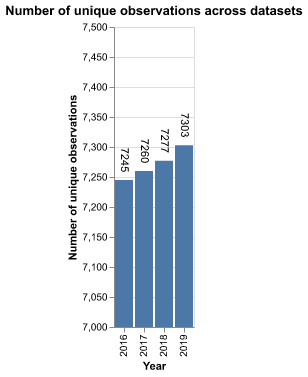
\includegraphics[width=3.20833in,height=3.92708in]{pset4_template_files/figure-pdf/cell-5-output-1.png}

\begin{verbatim}
b. The values are the same as on the previous data. This tells us that there are there are no repeated provider numbers in the data so we don't need to worry about repeat-values. Trend-wise, this tells us there is an increasing number of providers in each subsequent year.
\end{verbatim}

\subsection{Identify hospital closures in POS file (15 pts)
(*)}\label{identify-hospital-closures-in-pos-file-15-pts}

\begin{enumerate}
\def\labelenumi{\arabic{enumi}.}
\tightlist
\item
  There are 174 providers that fit this definition.
\end{enumerate}

\begin{Shaded}
\begin{Highlighting}[]
\CommentTok{\# create an empty df for facilities active in 2016 and closed by 2019}
\NormalTok{active2016\_closedby2019 }\OperatorTok{=}\NormalTok{ []}
\CommentTok{\# loop through all active providers in 2016 with provider number as reference}
\ControlFlowTok{for}\NormalTok{ active2016 }\KeywordTok{in}\NormalTok{ pos2016[}\StringTok{\textquotesingle{}PRVDR\_NUM\textquotesingle{}}\NormalTok{][pos2016[}\StringTok{\textquotesingle{}PGM\_TRMNTN\_CD\textquotesingle{}}\NormalTok{] }\OperatorTok{==} \DecValTok{0}\NormalTok{].unique():}
    \ControlFlowTok{for}\NormalTok{ year }\KeywordTok{in}\NormalTok{ [}\DecValTok{2017}\NormalTok{, }\DecValTok{2018}\NormalTok{, }\DecValTok{2019}\NormalTok{]:  }\CommentTok{\# loop through each year\textquotesingle{}s df}
        \ControlFlowTok{for}\NormalTok{ i, provider }\KeywordTok{in}\NormalTok{ pos\_combined[pos\_combined[}\StringTok{\textquotesingle{}YEAR\textquotesingle{}}\NormalTok{] }\OperatorTok{==}\NormalTok{ year].iterrows(): }\CommentTok{\# loop by provider in df (iterrows and i loop suggested by ChatGPT when debugging)}
            \ControlFlowTok{if}\NormalTok{ ((provider[}\StringTok{\textquotesingle{}PRVDR\_NUM\textquotesingle{}}\NormalTok{] }\OperatorTok{==}\NormalTok{ active2016) }\OperatorTok{\&}\NormalTok{ (provider[}\StringTok{\textquotesingle{}PGM\_TRMNTN\_CD\textquotesingle{}}\NormalTok{] }\OperatorTok{!=} \DecValTok{0}\NormalTok{) }\OperatorTok{\&}\NormalTok{ (active2016 }\KeywordTok{not} \KeywordTok{in}\NormalTok{ [entry[}\StringTok{\textquotesingle{}PRVDR\_NUM\textquotesingle{}}\NormalTok{] }\ControlFlowTok{for}\NormalTok{ entry }\KeywordTok{in}\NormalTok{ active2016\_closedby2019])):  }\CommentTok{\# looks for a provider number that matches the one we are referencing and it is not active and it is not already in our df}
\NormalTok{                active2016\_closedby2019.append(\{}
                    \StringTok{\textquotesingle{}PRVDR\_NUM\textquotesingle{}}\NormalTok{: active2016,}
                    \StringTok{\textquotesingle{}FAC\_NAME\textquotesingle{}}\NormalTok{: provider[}\StringTok{\textquotesingle{}FAC\_NAME\textquotesingle{}}\NormalTok{],}
                    \StringTok{\textquotesingle{}ZIP\_CD\textquotesingle{}}\NormalTok{: provider[}\StringTok{\textquotesingle{}ZIP\_CD\textquotesingle{}}\NormalTok{],}
                    \StringTok{\textquotesingle{}CLOSURE\_YEAR\textquotesingle{}}\NormalTok{: }\BuiltInTok{int}\NormalTok{(year)}
\NormalTok{                \})  }\CommentTok{\# adds its number, name, zip, and suspected closure year to our new df}
                
\NormalTok{active2016\_closedby2019\_df }\OperatorTok{=}\NormalTok{ pd.DataFrame(active2016\_closedby2019) }\CommentTok{\# not resetting index on purpose for Q3}

\BuiltInTok{print}\NormalTok{(}\BuiltInTok{len}\NormalTok{(active2016\_closedby2019\_df)) }\CommentTok{\# print num of observations}
\end{Highlighting}
\end{Shaded}

\begin{verbatim}
174
\end{verbatim}

\begin{enumerate}
\def\labelenumi{\arabic{enumi}.}
\setcounter{enumi}{1}
\tightlist
\item
\end{enumerate}

\begin{Shaded}
\begin{Highlighting}[]
\NormalTok{active2016\_closedby2019\_df.sort\_values(}\StringTok{\textquotesingle{}FAC\_NAME\textquotesingle{}}\NormalTok{).head(}\DecValTok{10}\NormalTok{)}
\end{Highlighting}
\end{Shaded}

\begin{longtable}[]{@{}lllll@{}}
\toprule\noalign{}
& PRVDR\_NUM & FAC\_NAME & ZIP\_CD & CLOSURE\_YEAR \\
\midrule\noalign{}
\endhead
\bottomrule\noalign{}
\endlastfoot
4 & 030001 & ABRAZO MARYVALE CAMPUS & 85031.0 & 2017 \\
10 & 050196 & ADVENTIST MEDICAL CENTER - CENTRAL VALLEY & 93230.0 &
2017 \\
97 & 360151 & AFFINITY MEDICAL CENTER & 44646.0 & 2018 \\
80 & 330189 & ALBANY MEDICAL CENTER / SOUTH CLINICAL CAMPUS & 12208.0 &
2017 \\
140 & 450488 & ALLEGIANCE SPECIALTY HOSPITAL OF KILGORE & 75662.0 &
2017 \\
62 & 250159 & ALLIANCE LAIRD HOSPITAL & 39365.0 & 2019 \\
101 & 370032 & ALLIANCEHEALTH DEACONESS & 73112.0 & 2019 \\
21 & 060036 & ARKANSAS VALLEY REGIONAL MEDICAL CENTER & 81050.0 &
2017 \\
156 & 520048 & ASCENSION NE WISCONSIN MERCY CAMPUS & 54904.0 & 2018 \\
88 & 340037 & ATRIUM HEALTH KINGS MOUNTAIN & 28086.0 & 2019 \\
\end{longtable}

\begin{enumerate}
\def\labelenumi{\arabic{enumi}.}
\setcounter{enumi}{2}
\tightlist
\item
  \begin{enumerate}
  \def\labelenumii{\alph{enumii}.}
  \tightlist
  \item
    165 hospitals fit this definition of potentially being a
    merger/acquisition.
  \end{enumerate}
\end{enumerate}

\begin{Shaded}
\begin{Highlighting}[]
\NormalTok{active2016\_closedby2019\_df\_dropped }\OperatorTok{=}\NormalTok{ active2016\_closedby2019\_df.copy() }\CommentTok{\# new df}
\NormalTok{dropped\_count }\OperatorTok{=} \DecValTok{0} \CommentTok{\# drop count}
\ControlFlowTok{for}\NormalTok{ index, row }\KeywordTok{in}\NormalTok{ active2016\_closedby2019\_df\_dropped.iterrows():}
\NormalTok{  len\_closure }\OperatorTok{=} \BuiltInTok{len}\NormalTok{(pos\_combined[(pos\_combined[}\StringTok{\textquotesingle{}ZIP\_CD\textquotesingle{}}\NormalTok{] }\OperatorTok{==}\NormalTok{ row[}\StringTok{\textquotesingle{}ZIP\_CD\textquotesingle{}}\NormalTok{]) }\OperatorTok{\&}\NormalTok{ (pos\_combined[}\StringTok{\textquotesingle{}YEAR\textquotesingle{}}\NormalTok{] }\OperatorTok{==}\NormalTok{ row[}\StringTok{\textquotesingle{}CLOSURE\_YEAR\textquotesingle{}}\NormalTok{])]) }\CommentTok{\# find num of providers in zip code year of suspected closure}
\NormalTok{  len\_before }\OperatorTok{=} \BuiltInTok{len}\NormalTok{(pos\_combined[(pos\_combined[}\StringTok{\textquotesingle{}ZIP\_CD\textquotesingle{}}\NormalTok{] }\OperatorTok{==}\NormalTok{ row[}\StringTok{\textquotesingle{}ZIP\_CD\textquotesingle{}}\NormalTok{]) }\OperatorTok{\&}\NormalTok{ (pos\_combined[}\StringTok{\textquotesingle{}YEAR\textquotesingle{}}\NormalTok{] }\OperatorTok{==}\NormalTok{ (row[}\StringTok{\textquotesingle{}CLOSURE\_YEAR\textquotesingle{}}\NormalTok{]}\OperatorTok{{-}}\DecValTok{1}\NormalTok{))]) }\CommentTok{\# find num of providers in zip code year before suspected closure}
  \ControlFlowTok{if}\NormalTok{ (len\_before }\OperatorTok{==}\NormalTok{ len\_closure): }\CommentTok{\# if num of hospitals is same}
\NormalTok{      active2016\_closedby2019\_df\_dropped }\OperatorTok{=}\NormalTok{ active2016\_closedby2019\_df\_dropped.drop(index) }\CommentTok{\# drop by index (this is why I didn\textquotesingle{}t reset index earlier)  }
\NormalTok{      dropped\_count }\OperatorTok{+=}\DecValTok{1} \CommentTok{\# update drop count}

\BuiltInTok{print}\NormalTok{(dropped\_count, }\StringTok{\textquotesingle{}hospitals fit this definition of potentially being a merger/acquisition.\textquotesingle{}}\NormalTok{)}
\end{Highlighting}
\end{Shaded}

\begin{verbatim}
165 hospitals fit this definition of potentially being a merger/acquisition.
\end{verbatim}

\begin{verbatim}
b. After correcting, there are 9 hospitals left.
\end{verbatim}

\begin{Shaded}
\begin{Highlighting}[]
\BuiltInTok{print}\NormalTok{(}\StringTok{\textquotesingle{}After correcting, there are\textquotesingle{}}\NormalTok{, }\BuiltInTok{len}\NormalTok{(active2016\_closedby2019\_df\_dropped), }\StringTok{\textquotesingle{}hospitals left.\textquotesingle{}}\NormalTok{)}
\end{Highlighting}
\end{Shaded}

\begin{verbatim}
After correcting, there are 9 hospitals left.
\end{verbatim}

\begin{verbatim}
c.
\end{verbatim}

\begin{Shaded}
\begin{Highlighting}[]
\NormalTok{active2016\_closedby2019\_df\_dropped.sort\_values(}\StringTok{\textquotesingle{}FAC\_NAME\textquotesingle{}}\NormalTok{).head(}\DecValTok{10}\NormalTok{)}
\end{Highlighting}
\end{Shaded}

\begin{longtable}[]{@{}lllll@{}}
\toprule\noalign{}
& PRVDR\_NUM & FAC\_NAME & ZIP\_CD & CLOSURE\_YEAR \\
\midrule\noalign{}
\endhead
\bottomrule\noalign{}
\endlastfoot
33 & 110187 & CHESTATEE REGIONAL HOSPITAL & 30533.0 & 2019 \\
103 & 370065 & CRAIG GENERAL HOSPITAL & 74301.0 & 2017 \\
149 & 450845 & EL PASO SPECIALTY HOSPITAL & 79902.0 & 2019 \\
118 & 400121 & HOSPITAL SAN GERARDO & 928.0 & 2017 \\
34 & 130067 & IDAHO DOCTORS HOSPITAL & 83221.0 & 2019 \\
16 & 050751 & MIRACLEMILE MEDICAL CENTER & 90036.0 & 2019 \\
42 & 180021 & PINEVILLE COMMUNITY HEALTH CENTER, INC & 40977.0 & 2019 \\
77 & 330108 & ST JOSEPH\textquotesingle S HOSPITAL & 14901.0 & 2019 \\
31 & 110039 & TRINITY HOSPITAL OF AUGUSTA & 30904.0 & 2018 \\
\end{longtable}

\subsection{Download Census zip code shapefile (10
pt)}\label{download-census-zip-code-shapefile-10-pt}

\begin{enumerate}
\def\labelenumi{\arabic{enumi}.}
\tightlist
\item
  \begin{enumerate}
  \def\labelenumii{\alph{enumii}.}
  \tightlist
  \item
    The five filetypes are a DBF (attribute information of the zip
    codes), a PRJ (describes the geocoordinate system being used, aka
    coordinate reference system, which in this case is specific to North
    America and uses degrees as distance units), an SHP (shapefile
    containing zip code geometric shapes), an SHX (has a positional
    index for where the zip codes are), and an xml (contains metadata
    about the dataset).
  \item
    The DBF file is \textasciitilde6425 KB, PRJ is 165 bytes, SHP is
    \textasciitilde837 MB, SHX is \textasciitilde265 KB, and XML is
    \textasciitilde15 KB, as printed below.
  \end{enumerate}
\end{enumerate}

\begin{Shaded}
\begin{Highlighting}[]
\ImportTok{import}\NormalTok{ os}
\ImportTok{from}\NormalTok{ os.path }\ImportTok{import}\NormalTok{ getsize}

\ControlFlowTok{for} \BuiltInTok{file} \KeywordTok{in}\NormalTok{ [}\StringTok{\textquotesingle{}dbf\textquotesingle{}}\NormalTok{, }\StringTok{\textquotesingle{}prj\textquotesingle{}}\NormalTok{, }\StringTok{\textquotesingle{}shp\textquotesingle{}}\NormalTok{, }\StringTok{\textquotesingle{}shx\textquotesingle{}}\NormalTok{, }\StringTok{\textquotesingle{}xml\textquotesingle{}}\NormalTok{]:}
\NormalTok{    path }\OperatorTok{=} \SpecialStringTok{f\textquotesingle{}C:/Users/amuly/OneDrive/Documents/GitHub/Python2{-}PS4/gz\_2010\_us\_860\_00\_500k/gz\_2010\_us\_860\_00\_500k.}\SpecialCharTok{\{}\BuiltInTok{file}\SpecialCharTok{\}}\SpecialStringTok{\textquotesingle{}}
    \BuiltInTok{print}\NormalTok{(}\BuiltInTok{file}\NormalTok{, os.path.getsize(path), }\StringTok{\textquotesingle{}bytes\textquotesingle{}}\NormalTok{) }\CommentTok{\#print file size in bytes for files extracted}
\end{Highlighting}
\end{Shaded}

\begin{verbatim}
dbf 6425474 bytes
prj 165 bytes
shp 837544580 bytes
shx 265060 bytes
xml 15639 bytes
\end{verbatim}

\begin{enumerate}
\def\labelenumi{\arabic{enumi}.}
\setcounter{enumi}{1}
\tightlist
\item
\end{enumerate}

\begin{Shaded}
\begin{Highlighting}[]
\ImportTok{import}\NormalTok{ geopandas }\ImportTok{as}\NormalTok{ gpd}

\NormalTok{shp\_path }\OperatorTok{=} \VerbatimStringTok{r"C:\textbackslash{}Users\textbackslash{}amuly\textbackslash{}OneDrive\textbackslash{}Documents\textbackslash{}GitHub\textbackslash{}Python2{-}PS4\textbackslash{}gz\_2010\_us\_860\_00\_500k/gz\_2010\_us\_860\_00\_500k.shp"}
\NormalTok{zip\_codes }\OperatorTok{=}\NormalTok{ gpd.read\_file(shp\_path)  }\CommentTok{\# import all zip codes}
\NormalTok{zip\_codes[}\StringTok{\textquotesingle{}ZIP\_INT\textquotesingle{}}\NormalTok{] }\OperatorTok{=}\NormalTok{ zip\_codes[}\StringTok{\textquotesingle{}ZCTA5\textquotesingle{}}\NormalTok{].}\BuiltInTok{apply}\NormalTok{(}
    \KeywordTok{lambda}\NormalTok{ g: }\BuiltInTok{int}\NormalTok{(g))  }\CommentTok{\# convert zips to int for comparison}
\NormalTok{texas\_zip\_codes }\OperatorTok{=}\NormalTok{ zip\_codes[(zip\_codes[}\StringTok{\textquotesingle{}ZIP\_INT\textquotesingle{}}\NormalTok{] }\OperatorTok{\textgreater{}=} \DecValTok{75000}\NormalTok{) }\OperatorTok{\&}\NormalTok{ (}
\NormalTok{    zip\_codes[}\StringTok{\textquotesingle{}ZIP\_INT\textquotesingle{}}\NormalTok{] }\OperatorTok{\textless{}} \DecValTok{80000}\NormalTok{)]  }\CommentTok{\# Texas zips start with 75{-}79}

\NormalTok{texas\_zip\_codes[}\StringTok{\textquotesingle{}PRVDR\_COUNT\textquotesingle{}}\NormalTok{] }\OperatorTok{=}\NormalTok{ texas\_zip\_codes[}\StringTok{\textquotesingle{}ZIP\_INT\textquotesingle{}}\NormalTok{].}\BuiltInTok{apply}\NormalTok{(}\KeywordTok{lambda}\NormalTok{ g: }\BuiltInTok{len}\NormalTok{(}
\NormalTok{    pos2016[pos2016[}\StringTok{\textquotesingle{}ZIP\_CD\textquotesingle{}}\NormalTok{] }\OperatorTok{==}\NormalTok{ g]))  }\CommentTok{\# column with 2016 provider counts by zip code}

\CommentTok{\# plot provider count by zip. Had a hard time choosing color scheme, but chose this one because black=0 was visually useful.}
\NormalTok{texas\_zip\_codes.plot(column}\OperatorTok{=}\StringTok{\textquotesingle{}PRVDR\_COUNT\textquotesingle{}}\NormalTok{, cmap}\OperatorTok{=}\StringTok{\textquotesingle{}gnuplot\textquotesingle{}}\NormalTok{, legend}\OperatorTok{=}\VariableTok{True}\NormalTok{, legend\_kwds}\OperatorTok{=}\NormalTok{\{}
                     \StringTok{\textquotesingle{}label\textquotesingle{}}\NormalTok{: }\StringTok{\textquotesingle{}Number of providers (2016)\textquotesingle{}}\NormalTok{\}).set\_axis\_off() }\CommentTok{\#plot provider count by zip. Had a hard time choosing color scheme, but chose this one because black=0 was visually useful.}
\end{Highlighting}
\end{Shaded}

\includegraphics{pset4_template_files/figure-pdf/cell-12-output-1.pdf}

\subsection{Calculate zip code's distance to the nearest hospital (20
pts)
(*)}\label{calculate-zip-codes-distance-to-the-nearest-hospital-20-pts}

\begin{enumerate}
\def\labelenumi{\arabic{enumi}.}
\tightlist
\item
  zip\_all\_centroids has 33,120 observations and 6 columns/attributes.
  The GEO\_ID column is the Census Bureau's identifier for this location
  (Source), the ZCTA5 column is the zip code tabulation area in 5 digits
  (Source), the NAME is the name of the area (in this case the zip code
  itself), the CENSUSAREA is the land area in square miles, and geometry
  is the polygon/multipolygon of the zip code upon which the centroid is
  calculated. Source:
  https://www.census.gov/programs-surveys/geography/guidance/geo-identifiers.html
\end{enumerate}

\begin{Shaded}
\begin{Highlighting}[]
\NormalTok{shx\_path }\OperatorTok{=} \VerbatimStringTok{r"C:\textbackslash{}Users\textbackslash{}amuly\textbackslash{}OneDrive\textbackslash{}Documents\textbackslash{}GitHub\textbackslash{}Python2{-}PS4\textbackslash{}gz\_2010\_us\_860\_00\_500k/gz\_2010\_us\_860\_00\_500k.shx"}
\NormalTok{zip\_all\_centroids }\OperatorTok{=}\NormalTok{ gpd.read\_file(shx\_path) }
\NormalTok{zip\_all\_centroids.shape}
\end{Highlighting}
\end{Shaded}

\begin{verbatim}
(33120, 6)
\end{verbatim}

\begin{enumerate}
\def\labelenumi{\arabic{enumi}.}
\setcounter{enumi}{1}
\tightlist
\item
  There are 1935 unique values in the Texas subset, and 4057 in the
  Texas + bordering states subset.
\end{enumerate}

\begin{Shaded}
\begin{Highlighting}[]
\NormalTok{zip\_all\_centroids[}\StringTok{\textquotesingle{}ZIP\_INT\textquotesingle{}}\NormalTok{] }\OperatorTok{=}\NormalTok{ zip\_all\_centroids[}\StringTok{\textquotesingle{}ZCTA5\textquotesingle{}}\NormalTok{].}\BuiltInTok{apply}\NormalTok{(}
    \KeywordTok{lambda}\NormalTok{ g: }\BuiltInTok{int}\NormalTok{(g))  }\CommentTok{\# convert zips to int for comparison}
\NormalTok{zips\_texas\_centroids }\OperatorTok{=}\NormalTok{ zip\_all\_centroids[(zip\_all\_centroids[}\StringTok{\textquotesingle{}ZIP\_INT\textquotesingle{}}\NormalTok{] }\OperatorTok{\textgreater{}=} \DecValTok{75000}\NormalTok{) }\OperatorTok{\&}\NormalTok{ (}
\NormalTok{    zip\_all\_centroids[}\StringTok{\textquotesingle{}ZIP\_INT\textquotesingle{}}\NormalTok{] }\OperatorTok{\textless{}} \DecValTok{80000}\NormalTok{)]  }\CommentTok{\# Texas zips start with 75{-}79}
\NormalTok{zips\_texas\_borderstates\_centroids }\OperatorTok{=}\NormalTok{ zip\_all\_centroids[}
\NormalTok{    ((zip\_all\_centroids[}\StringTok{\textquotesingle{}ZIP\_INT\textquotesingle{}}\NormalTok{] }\OperatorTok{\textgreater{}=} \DecValTok{70000}\NormalTok{)}
     \OperatorTok{\&}\NormalTok{ (zip\_all\_centroids[}\StringTok{\textquotesingle{}ZIP\_INT\textquotesingle{}}\NormalTok{] }\OperatorTok{\textless{}} \DecValTok{80000}\NormalTok{))     }\CommentTok{\# covers Texas 75{-}79, Louisiana 700{-}715, Arkanasas 716{-}729, Oklahama 73{-}74}
    \OperatorTok{|}\NormalTok{ (}
\NormalTok{        (zip\_all\_centroids[}\StringTok{\textquotesingle{}ZIP\_INT\textquotesingle{}}\NormalTok{] }\OperatorTok{\textgreater{}=} \DecValTok{87000}\NormalTok{)}
         \OperatorTok{\&}\NormalTok{ (zip\_all\_centroids[}\StringTok{\textquotesingle{}ZIP\_INT\textquotesingle{}}\NormalTok{] }\OperatorTok{\textless{}} \DecValTok{88500}\NormalTok{)  }\CommentTok{\# covers New Mexico 870{-}884}
\NormalTok{    )]}

\BuiltInTok{print}\NormalTok{(zips\_texas\_centroids[}\StringTok{\textquotesingle{}ZIP\_INT\textquotesingle{}}\NormalTok{].nunique())}
\BuiltInTok{print}\NormalTok{(zips\_texas\_borderstates\_centroids[}\StringTok{\textquotesingle{}ZIP\_INT\textquotesingle{}}\NormalTok{].nunique())}
\CommentTok{\# skipped extra credit}
\end{Highlighting}
\end{Shaded}

\begin{verbatim}
1935
4057
\end{verbatim}

\begin{enumerate}
\def\labelenumi{\arabic{enumi}.}
\setcounter{enumi}{2}
\tightlist
\item
  This should be an inner merge, because we only want to keep zip codes
  with hospitals from our other dataset, and only bring in hospitals
  that are in our zip code dataset. I merged on
  zips\_texas\_borderstates\_centroid's ZIP\_INT variable I made earlier
  with the zip codes as int, and my 2016 dataset's ZIP\_CD variable.
\end{enumerate}

\begin{Shaded}
\begin{Highlighting}[]
\NormalTok{zips\_withhospital\_centroids }\OperatorTok{=}\NormalTok{ zips\_texas\_borderstates\_centroids.merge(pos2016, left\_on}\OperatorTok{=}\StringTok{\textquotesingle{}ZIP\_INT\textquotesingle{}}\NormalTok{, right\_on}\OperatorTok{=}\StringTok{\textquotesingle{}ZIP\_CD\textquotesingle{}}\NormalTok{, how}\OperatorTok{=}\StringTok{\textquotesingle{}inner\textquotesingle{}}\NormalTok{)}
\end{Highlighting}
\end{Shaded}

\begin{enumerate}
\def\labelenumi{\arabic{enumi}.}
\setcounter{enumi}{3}
\tightlist
\item
  \begin{enumerate}
  \def\labelenumii{\alph{enumii}.}
  \tightlist
  \item
    Running the code for the first ten rows took 0.2 seconds. With a
    dataset of 1935 observations this would take approximately 38.7
    seconds.
  \item
    When running the whole thing, it actually took 17.1 seconds.
  \end{enumerate}
\end{enumerate}

\begin{Shaded}
\begin{Highlighting}[]
\CommentTok{\# PART A AND B CODE}
\NormalTok{zips\_texas\_centroids[}\StringTok{\textquotesingle{}PRVDR\_DIST\textquotesingle{}}\NormalTok{] }\OperatorTok{=} \VariableTok{None}  \CommentTok{\# New column for nearest provider}
\NormalTok{zips\_texas\_centroids[}\StringTok{\textquotesingle{}centroid\textquotesingle{}}\NormalTok{] }\OperatorTok{=}\NormalTok{ zips\_texas\_centroids.geometry.centroid }\CommentTok{\# add centroid column}
\NormalTok{zips\_withhospital\_centroids[}\StringTok{\textquotesingle{}centroid\textquotesingle{}}\NormalTok{] }\OperatorTok{=}\NormalTok{ zips\_withhospital\_centroids.geometry.centroid }\CommentTok{\# add centroid column}
\CommentTok{\#\%timeit}
\CommentTok{\# removed the first ten rows test:}
\CommentTok{\# for index, row in zips\_texas\_centroids[0:10].iterrows():}
\ControlFlowTok{for}\NormalTok{ index, row }\KeywordTok{in}\NormalTok{ zips\_texas\_centroids.iterrows():}
\NormalTok{    zip\_texas }\OperatorTok{=}\NormalTok{ row[}\StringTok{\textquotesingle{}centroid\textquotesingle{}}\NormalTok{]}
    \ControlFlowTok{if}\NormalTok{ row[}\StringTok{\textquotesingle{}ZIP\_INT\textquotesingle{}}\NormalTok{] }\KeywordTok{in}\NormalTok{ zips\_withhospital\_centroids[}\StringTok{\textquotesingle{}ZIP\_INT\textquotesingle{}}\NormalTok{]: }\CommentTok{\# first check if it has a provider}
\NormalTok{        zips\_texas\_centroids.at[index, }\StringTok{\textquotesingle{}PRVDR\_DIST\textquotesingle{}}\NormalTok{] }\OperatorTok{=} \DecValTok{0} \CommentTok{\# if so the distance is zero, and skip to next row}
        \ControlFlowTok{continue}
    \ControlFlowTok{else}\NormalTok{:}
\NormalTok{        distances }\OperatorTok{=}\NormalTok{ [zip\_texas.distance(}
\NormalTok{        zip\_hospital) }\ControlFlowTok{for}\NormalTok{ zip\_hospital }\KeywordTok{in}\NormalTok{ zips\_withhospital\_centroids[}\StringTok{\textquotesingle{}centroid\textquotesingle{}}\NormalTok{]] }\CommentTok{\# list of distances to zip codes with hospitals}
\NormalTok{        zips\_texas\_centroids.at[index, }\StringTok{\textquotesingle{}PRVDR\_DIST\textquotesingle{}}\NormalTok{] }\OperatorTok{=} \BuiltInTok{min}\NormalTok{(distances) }\CommentTok{\# add smallest distance to column}
\end{Highlighting}
\end{Shaded}

\begin{verbatim}
c.  The prj file says it is using degrees. I used the conversion of 1 degree to 69 miles.
\end{verbatim}

\begin{Shaded}
\begin{Highlighting}[]
\CommentTok{\# PART C CODE}
\NormalTok{zips\_texas\_centroids[}\StringTok{\textquotesingle{}PRVDR\_DIST\_MILES\textquotesingle{}}\NormalTok{] }\OperatorTok{=}\NormalTok{ zips\_texas\_centroids[}\StringTok{\textquotesingle{}PRVDR\_DIST\textquotesingle{}}\NormalTok{]}\OperatorTok{*}\DecValTok{69} \CommentTok{\# converting to miles}
\end{Highlighting}
\end{Shaded}

\begin{enumerate}
\def\labelenumi{\arabic{enumi}.}
\setcounter{enumi}{4}
\tightlist
\item
  \begin{enumerate}
  \def\labelenumii{\alph{enumii}.}
  \tightlist
  \item
    The mean is 0.12842963890434103 degrees.
  \end{enumerate}
\end{enumerate}

\begin{Shaded}
\begin{Highlighting}[]
\CommentTok{\#PART A CODE}
\BuiltInTok{print}\NormalTok{(zips\_texas\_centroids[}\StringTok{\textquotesingle{}PRVDR\_DIST\textquotesingle{}}\NormalTok{].mean())}
\end{Highlighting}
\end{Shaded}

\begin{verbatim}
0.12842963890434103
\end{verbatim}

\begin{verbatim}
b. The mean is 8.86164508439954 miles. This makes sense as hospitals tend to be within driving distance on average. It is likely this high because it is skewed right by some remote zip codes.
\end{verbatim}

\begin{Shaded}
\begin{Highlighting}[]
\CommentTok{\#PART B CODE}
\BuiltInTok{print}\NormalTok{(zips\_texas\_centroids[}\StringTok{\textquotesingle{}PRVDR\_DIST\_MILES\textquotesingle{}}\NormalTok{].mean())}
\end{Highlighting}
\end{Shaded}

\begin{verbatim}
8.86164508439954
\end{verbatim}

\begin{verbatim}
c.
\end{verbatim}

\begin{Shaded}
\begin{Highlighting}[]
\CommentTok{\#PART C CODE}
\NormalTok{zips\_texas\_centroids[}\StringTok{\textquotesingle{}PRVDR\_DIST\_MILES\textquotesingle{}}\NormalTok{] }\OperatorTok{=}\NormalTok{ pd.to\_numeric(zips\_texas\_centroids[}\StringTok{\textquotesingle{}PRVDR\_DIST\_MILES\textquotesingle{}}\NormalTok{], errors}\OperatorTok{=}\StringTok{\textquotesingle{}coerce\textquotesingle{}}\NormalTok{) }\CommentTok{\# fixed error preventing me from plotting legend}

\NormalTok{zips\_texas\_centroids.plot(column}\OperatorTok{=}\StringTok{\textquotesingle{}PRVDR\_DIST\_MILES\textquotesingle{}}\NormalTok{, cmap}\OperatorTok{=}\StringTok{\textquotesingle{}rainbow\textquotesingle{}}\NormalTok{, legend}\OperatorTok{=}\VariableTok{True}\NormalTok{, legend\_kwds}\OperatorTok{=}\NormalTok{\{}\StringTok{\textquotesingle{}label\textquotesingle{}}\NormalTok{: }\StringTok{\textquotesingle{}Miles to nearest hospital (2016)\textquotesingle{}}\NormalTok{\}).set\_axis\_off() }\CommentTok{\# plotted}
\end{Highlighting}
\end{Shaded}

\includegraphics{pset4_template_files/figure-pdf/cell-20-output-1.pdf}

\subsection{Effects of closures on access in Texas (15
pts)}\label{effects-of-closures-on-access-in-texas-15-pts}

\begin{enumerate}
\def\labelenumi{\arabic{enumi}.}
\tightlist
\item
\end{enumerate}

\begin{Shaded}
\begin{Highlighting}[]
\NormalTok{pd.set\_option(}\StringTok{\textquotesingle{}display.max\_rows\textquotesingle{}}\NormalTok{, }\VariableTok{None}\NormalTok{)}
\NormalTok{active2016\_closedby2019\_df\_counts }\OperatorTok{=}\NormalTok{ active2016\_closedby2019\_df[}\StringTok{\textquotesingle{}ZIP\_CD\textquotesingle{}}\NormalTok{].value\_counts(}
\NormalTok{).reset\_index()}
\NormalTok{active2016\_closedby2019\_df\_counts[}\StringTok{\textquotesingle{}ZIP\_CD\textquotesingle{}}\NormalTok{] }\OperatorTok{=}\NormalTok{ active2016\_closedby2019\_df\_counts[}\StringTok{\textquotesingle{}ZIP\_CD\textquotesingle{}}\NormalTok{].}\BuiltInTok{apply}\NormalTok{(}
    \KeywordTok{lambda}\NormalTok{ g: }\BuiltInTok{int}\NormalTok{(g))}
\NormalTok{active2016\_closedby2019\_df\_texas\_counts }\OperatorTok{=}\NormalTok{ active2016\_closedby2019\_df\_counts[active2016\_closedby2019\_df\_counts[}\StringTok{\textquotesingle{}ZIP\_CD\textquotesingle{}}\NormalTok{].isin(}
\NormalTok{    zips\_texas\_centroids[}\StringTok{\textquotesingle{}ZIP\_INT\textquotesingle{}}\NormalTok{])].reset\_index()}
\BuiltInTok{print}\NormalTok{(active2016\_closedby2019\_df\_texas\_counts)}
\end{Highlighting}
\end{Shaded}

\begin{verbatim}
    index  ZIP_CD  count
0     131   76502      1
1     132   75601      1
2     133   79735      1
3     134   76645      1
4     135   79520      1
5     136   75042      1
6     137   78061      1
7     138   79553      1
8     139   75662      1
9     140   75835      1
10    141   78336      1
11    142   78834      1
12    143   77065      1
13    144   79529      1
14    145   75862      1
15    146   76531      1
16    147   75390      1
17    148   79902      1
18    149   75235      1
19    159   77054      1
20    160   77429      1
21    161   77479      1
22    162   77035      1
23    163   78734      1
24    164   75051      1
25    165   78613      1
26    166   78017      1
27    167   75231      1
28    168   76520      1
29    169   77598      1
30    170   75087      1
31    171   79761      1
32    172   75140      1
\end{verbatim}

\begin{enumerate}
\def\labelenumi{\arabic{enumi}.}
\setcounter{enumi}{1}
\tightlist
\item
  There are 33 zip codes that were directly affected.
\end{enumerate}

\begin{Shaded}
\begin{Highlighting}[]
\NormalTok{active2016\_closedby2019\_df\_counts[}\StringTok{\textquotesingle{}ZIP\_INT\textquotesingle{}}\NormalTok{] }\OperatorTok{=}\NormalTok{ active2016\_closedby2019\_df\_counts[}\StringTok{\textquotesingle{}ZIP\_CD\textquotesingle{}}\NormalTok{].}\BuiltInTok{apply}\NormalTok{(}
    \KeywordTok{lambda}\NormalTok{ g: }\BuiltInTok{int}\NormalTok{(g))}
\NormalTok{zips\_texas\_centroids }\OperatorTok{=}\NormalTok{ zips\_texas\_centroids.merge(}
\NormalTok{    active2016\_closedby2019\_df\_texas\_counts, left\_on}\OperatorTok{=}\StringTok{\textquotesingle{}ZIP\_INT\textquotesingle{}}\NormalTok{, right\_on}\OperatorTok{=}\StringTok{\textquotesingle{}ZIP\_CD\textquotesingle{}}\NormalTok{, how}\OperatorTok{=}\StringTok{\textquotesingle{}left\textquotesingle{}}\NormalTok{)}

\NormalTok{zips\_texas\_centroids[}\StringTok{\textquotesingle{}count\textquotesingle{}}\NormalTok{].fillna(}\DecValTok{0}\NormalTok{, inplace}\OperatorTok{=}\VariableTok{True}\NormalTok{)}
\CommentTok{\# filled missing counts as zero}

\NormalTok{zips\_texas\_centroids.plot(column}\OperatorTok{=}\StringTok{\textquotesingle{}count\textquotesingle{}}\NormalTok{, legend}\OperatorTok{=}\VariableTok{True}\NormalTok{, legend\_kwds}\OperatorTok{=}\NormalTok{\{}
                          \StringTok{\textquotesingle{}label\textquotesingle{}}\NormalTok{: }\StringTok{\textquotesingle{}Hospitals closed 2017{-}2019\textquotesingle{}}\NormalTok{\}).set\_axis\_off() }\CommentTok{\# plotted}

\BuiltInTok{print}\NormalTok{(}\BuiltInTok{len}\NormalTok{(zips\_texas\_centroids[zips\_texas\_centroids[}\StringTok{\textquotesingle{}count\textquotesingle{}}\NormalTok{] }\OperatorTok{\textgreater{}} \DecValTok{0}\NormalTok{])) }\CommentTok{\# number of zip codes with a closed hospital}
\end{Highlighting}
\end{Shaded}

\begin{verbatim}
33
\end{verbatim}

\includegraphics{pset4_template_files/figure-pdf/cell-22-output-2.pdf}

\begin{enumerate}
\def\labelenumi{\arabic{enumi}.}
\setcounter{enumi}{2}
\tightlist
\item
  There are 231 zip codes in total that were affected, subtracting the
  33 directly affected from above we get 198 specifically indirectly
  affected.
\end{enumerate}

\begin{Shaded}
\begin{Highlighting}[]
\NormalTok{directly\_affected }\OperatorTok{=}\NormalTok{ zips\_texas\_centroids[zips\_texas\_centroids[}\StringTok{\textquotesingle{}count\textquotesingle{}}\NormalTok{] }\OperatorTok{\textgreater{}} \DecValTok{0}\NormalTok{] }\CommentTok{\# geo df with directly affected zip codes}
\NormalTok{directly\_affected[}\StringTok{\textquotesingle{}buffer\textquotesingle{}}\NormalTok{] }\OperatorTok{=}\NormalTok{ directly\_affected.geometry.}\BuiltInTok{buffer}\NormalTok{((}\DecValTok{10}\OperatorTok{/}\DecValTok{69}\NormalTok{)) }\CommentTok{\# add buffer with degree conversion}
\NormalTok{indirectly\_affected }\OperatorTok{=}\NormalTok{ gpd.sjoin(directly\_affected, zips\_texas\_centroids, how}\OperatorTok{=}\StringTok{"inner"}\NormalTok{, predicate}\OperatorTok{=}\StringTok{"intersects"}\NormalTok{)}
\BuiltInTok{print}\NormalTok{(}\BuiltInTok{len}\NormalTok{(indirectly\_affected))}
\end{Highlighting}
\end{Shaded}

\begin{verbatim}
231
\end{verbatim}

\begin{enumerate}
\def\labelenumi{\arabic{enumi}.}
\setcounter{enumi}{3}
\tightlist
\item
\end{enumerate}

\begin{Shaded}
\begin{Highlighting}[]
\NormalTok{zips\_texas\_centroids[}\StringTok{\textquotesingle{}affected\textquotesingle{}}\NormalTok{] }\OperatorTok{=} \VariableTok{None} \CommentTok{\# create col to hold affected variable}
\ControlFlowTok{for}\NormalTok{ index, row }\KeywordTok{in}\NormalTok{ zips\_texas\_centroids.iterrows():}
    \ControlFlowTok{if}\NormalTok{ row[}\StringTok{\textquotesingle{}count\textquotesingle{}}\NormalTok{] }\OperatorTok{\textgreater{}} \DecValTok{0}\NormalTok{: }\CommentTok{\# first check if directly affected}
\NormalTok{        zips\_texas\_centroids.at[index, }\StringTok{\textquotesingle{}affected\textquotesingle{}}\NormalTok{] }\OperatorTok{=} \StringTok{"Directly"}
        \ControlFlowTok{continue}
    \ControlFlowTok{elif}\NormalTok{ row[}\StringTok{\textquotesingle{}ZIP\_INT\textquotesingle{}}\NormalTok{] }\KeywordTok{in}\NormalTok{ indirectly\_affected[}\StringTok{\textquotesingle{}ZIP\_INT\_right\textquotesingle{}}\NormalTok{].values: }\CommentTok{\# else check if brought onto indirectly\_affected}
\NormalTok{        zips\_texas\_centroids.at[index, }\StringTok{\textquotesingle{}affected\textquotesingle{}}\NormalTok{] }\OperatorTok{=} \StringTok{"Indirectly"}
        \ControlFlowTok{continue}
    \ControlFlowTok{else}\NormalTok{: }\CommentTok{\# else it is unaffected}
\NormalTok{        zips\_texas\_centroids.at[index, }\StringTok{\textquotesingle{}affected\textquotesingle{}}\NormalTok{] }\OperatorTok{=} \StringTok{"Unaffected"}
        \ControlFlowTok{continue}
\NormalTok{zips\_texas\_centroids.plot(column}\OperatorTok{=}\StringTok{\textquotesingle{}affected\textquotesingle{}}\NormalTok{, cmap }\OperatorTok{=} \StringTok{\textquotesingle{}copper\textquotesingle{}}\NormalTok{, legend}\OperatorTok{=}\VariableTok{True}\NormalTok{, legend\_kwds}\OperatorTok{=}\NormalTok{\{}\StringTok{\textquotesingle{}title\textquotesingle{}}\NormalTok{: }\StringTok{\textquotesingle{}Affected by closure\textquotesingle{}}\NormalTok{, }\StringTok{\textquotesingle{}loc\textquotesingle{}}\NormalTok{: }\StringTok{\textquotesingle{}lower left\textquotesingle{}}\NormalTok{, }\StringTok{\textquotesingle{}fontsize\textquotesingle{}}\NormalTok{:}\StringTok{\textquotesingle{}small\textquotesingle{}}\NormalTok{\}).set\_axis\_off()}
\end{Highlighting}
\end{Shaded}

\includegraphics{pset4_template_files/figure-pdf/cell-24-output-1.pdf}

\subsection{Reflecting on the exercise (10
pts)}\label{reflecting-on-the-exercise-10-pts}

\begin{enumerate}
\def\labelenumi{\arabic{enumi}.}
\item
  If we look at the data dictionary, we can see there are many reasons a
  program termination code may change, not just because of a
  merger/acquisition. Our code is imperfect because it firstly assumes
  anything missing or with a non ``0'' code is closed, secondly because
  it only accounts for mergers when correcting this assumption via zip
  codes. Our methods could be improved by cross-checking facility names
  and provider numbers year-to-year (as opposed to just seeing if the
  number of providers changes) and by accounting for the other
  variations of termination codes that might not really be terminations.
\item
  We consider zip-codes affected by closures by determining which zip
  codes are within a ten mile radius of a zip code with a closure. This
  is somewhat useful, but it makes the assumption that the closure only
  affects people intersecting with that buffer. However, if this was the
  only hospital in a bordering zip code (earlier we saw some zips had a
  20+ mile distance to nearest hospital), that would make them directly
  affected. So, I would first add a definition to directly affected to
  include zips whose nearest hospital was in the zip code with the
  closure, to show the true effect on these more remote communities.
  Secondly, it would be useful to add a degree of affectedness; if there
  are 20 hospitals in a zip and one closes, this is not as much of an
  affect as if it was the only hospital. If not turning it into a scale
  (proportion of 2016 hospitals in a zip that remain open, for example)
  then we could introduce an additional value, like `Totally' affected,
  to represent zips where the only hospital or nearest hospital closed.
\end{enumerate}




\end{document}
